% Chapter 1

\chapter{Quantum Embedding}
\label{chapter:quantum_embedding} % Main chapter title

%----------------------------------------------------------------------------------------

% Define some commands to keep the formatting separated from the content 

%comment these back in when you remove Chapter0 from the document

%\newcommand{\keyword}[1]{\textbf{#1}}
%\newcommand{\tabhead}[1]{\textbf{#1}}
%\newcommand{\code}[1]{\texttt{#1}}
%\newcommand{\file}[1]{\texttt{\bfseries#1}}
%\newcommand{\option}[1]{\texttt{\itshape#1}}

%----------------------------------------------------------------------------------------

\section{Quantum Data Encoding}\label{section:quantum_data_encoding}
Quantum data encoding or quantum data embedding\footnote{The terms \textit{encoding} and \textit{embedding} can be used interchangeably in this context.} describes the process of loading classical data in a quantum circuit by encoding it into the state of the qubits. In fact, the classical data is encoded in a Hilbert space using a quantum feature map. Lloyd et al.\cite{Quantum_embeddings_for_machine_learning_2020} defines quantum embedding as a quantum state $\ket{x}$ that represents a data input $x \in X$. It is facilitated by a quantum feature map $\phi : x \rightarrow \ket{x}$. For example, the quantum feature map can be executed by a quantum circuit $\Phi(x)$ whose gate parameters depend on $x$.

There are multiple ways of encoding classical data onto quantum states (see list \ref{list:encoding_patterns}) using a quantum feature map which directly affects the computational power of the quantum circuit, emphasizing that the encoding is a crucial part in designing quantum algorithms.\cite{Quantum_machine_learning_in_feature_Hilbert_spaces_2019,Supervised_learning_with_quantum-enhanced_feature_spaces_2019,Quantum_embeddings_for_machine_learning_2020,PennyLane_QuantumEmbedding,PennyLane_QuantumFeatureMap,schuld2021supervised,leymann2019pattern}\par
\par
\noindent An incomplete list of encoding patterns for quantum algorithms\cite{schuld2021supervised,Weigold2021_ExpandingDataEncodingPatterns,leymann2019pattern}: \label{list:encoding_patterns}
\begin{itemize}
    \item Basis Encoding (See section \ref{section:basis_embedding})
    \item Angle Encoding or Tensor Product Encoding (See section \ref{section:angle_embedding}) \cite{leymannBitterTruthGatebased2020}
    \item Amplitude Encoding \& Repeated Amplitude Encoding
    \item Quantum Associative Memory (QUAM) Encoding
    \item Quantum Random Access Memory (QRAM) Encoding \\\textit{(No hardware implementation of QRAM exists until today \cite{Weigold2021_ExpandingDataEncodingPatterns})}
    \item Coherent State Encoding
    \item General Near-term Encoding
    \item Divide‑and‑conquer Encoding \cite{araujoDivideandconquerAlgorithmQuantum2021}
\end{itemize}

\subsection{State Preparation (Initialization)}\label{subsection:state_preparation}

The section in a quantum circuit where the classical data encoding is initialized is referred to as \textit{state preparation}\cite{leymann2019pattern,Weigold2021_ExpandingDataEncodingPatterns} (see figure \ref{fig:circuit_state_preparation}) and can consist of multiple different gates depending on the requirements of the chosen encoding and the quantum algorithm. 

\begin{figure}[!h]
    \centering
    \scalebox{1.0}{
        \Qcircuit @C=1em @R=.7em {
            \nghost{ {q}_{0} :  } & \lstick{ {q}_{0} :  } & \multigate{2}{state\break{}preparation} & \rstick{\cdots} \qw \\
            \nghost{ {q}_{1} :  } & \lstick{ {q}_{1} :  } & \ghost{state\break{}preparation} & \rstick{\cdots} \qw \\
            \nghost{ {q}_{2} :  } & \lstick{ {q}_{2} :  } & \ghost{state\break{}preparation} & \rstick{\cdots} \qw
        }
    }
    \caption{Abstract example quantum circuit with 3 qubits which encodes classical data and starts with a \textit{state preparation} routine}
    \label{fig:circuit_state_preparation}
\end{figure}

There is a trade-off between the following three major criteria\cite{Weigold2021_ExpandingDataEncodingPatterns}:
\begin{itemize}
    \item \textit{The amount of qubits needed for the encoding should be minimal} because current devices are of intermediate size and thus only contain a limited amount of qubits
    \item \textit{The number of parallel operations needed to realize the encoding should be minimal to minimize the width of the quantum circuit} - ideally, the loading routine is of constant or logarithmic complexity
    \item \textit{The data must be represented in a suitable manner} for further calculations, e.g., arithmetic operations.
\end{itemize}

\section{Basis Embedding}\label{section:basis_embedding}

The main idea of basis embedding is to encode a real number, approximated by a binary format, into the computational basis $\{\ket{0…00}, \ket{0…01}, …, \ket{1…11}\}$ of the quantum state. For example, the number "$5$" (decimal) is represented as $101$ (binary format) which is then encoded by $\ket{101}$\cite{Weigold2021_EncodingPatternsForQuantumAlgorithms,schuld2021supervised}. The $\mathrm{X}$ gate (see section \ref{chapter:basic_opterations}) is used to set a qubit with initial ground state $\ket{0}$ to $\ket{1}$ as shown in figure \ref{fig:basis_embedding_example}.

\begin{figure}[!h]
    \centering
    \scalebox{0.9}{
        \begin{tikzpicture}[
          squarednode/.style={rectangle, draw=white!60, fill=white!5, thick, minimum size=15mm}
        ]
            %Nodes
            \node[squarednode] (number)                                {$5_d = 101_b$};
            \node              (placeholder)    [right=of number]      {};
            \node              (quantumcircuit) [right=of placeholder] {
                \Qcircuit @C=1em @R=.7em {
                    \lstick{\ket{0}} & \gate{X} & \rstick{\ket{1}} \qw \\
                    \lstick{\ket{0}} & \qw & \rstick{\ket{0}} \qw \\
                    \lstick{\ket{0}} & \gate{X} & \rstick{\ket{1}} \qw 
                }
            };
            \node              (placeholder2)  [right=of quantumcircuit] {};
            \node[squarednode] (state)         [right=of placeholder2]   {$\ket{101}$};
            % Lines
            \draw[->] (number.east) -- ++(1.25,0);
            \draw[->] (quantumcircuit.east) + (0.75,0) -- (state.west);
            % \draw [->] (optimizer.north) -- ++(0,+1.25) -- ++(-6.15,0) node[auto,midway,above] {updates} -| ++(0,-1);
        \end{tikzpicture}
    }
    \caption{Basis encoding quantum circuit example with $\mathrm{X}$ gates to encode the decimal number $5$ represented as $101_b$ into the quantum state}
    \label{fig:basis_embedding_example}
\end{figure}

\section{Angle Embedding}\label{section:angle_embedding}

Whilst angle embedding is not optimal as it requires $n$ qubits to represent $n$-dimensional data, it is efficient regarding operations and directly useful for processing data in quantum neural networks\cite{Weigold2021_ExpandingDataEncodingPatterns,leymannBitterTruthGatebased2020}. Weigold et al. state that only single-qubit rotations are needed for the state preparation routine, which is highly efficient and can be done in parallel for each qubit. \par
The experiments are limited to angle encoding in the quantum circuits, where the value is directly encoded onto the rotation angle of the qubit state. Parametrizable gates\cite{qiskit_rygate_nodate} are used for the encoding. A detailed explanation of the used $\mathrm{RY}(\theta)$ gate is available in chapter \ref{chapter:rotations} \par
 
Consider the example in figure \ref{fig:example_encoding_circuit_ry} where the features $x, y$ are angle encoded onto the qubits $q_0, q_1$ using the $\mathrm{RY}(\theta)$ rotation gate, where $\theta$ is replaced with the corresponding feature. 

\begin{figure}[!h]
    \centering
    \scalebox{1.0}{
        \Qcircuit @C=1.0em @R=1.0em @!R { 
            \nghost{ {q}_{0} :  } & \lstick{ {q}_{0} :  } & \gate{\mathrm{R_Y}\,(1.25)} & \qw & \qw\\ 
            \nghost{ {q}_{1} :  } & \lstick{ {q}_{1} :  } & \gate{\mathrm{R_Y}\,(2.3)} & \qw & \qw  \gategroup{1}{3}{2}{3}{.7em}{--}\\ 
        }
    }
    \caption{Angle encoding quantum circuit example with $\mathrm{RY}$ gates and grouping around the \textit{state preparation}}
    \label{fig:example_encoding_circuit_ry}
\end{figure}

The corresponding quantum state equation (\ref{equation:angle_embedding_two_hadamard_example}), as shown by Weigold et al.\cite{Weigold2021_ExpandingDataEncodingPatterns}:

\begin{equation}
    \centering
    \begin{split}
        \ket{\psi} &=\ \begin{pmatrix}\cos{\frac{1.25}{2}} \\ \sin{\frac{1.25}{2}}\end{pmatrix} \otimes \begin{pmatrix}\cos{\frac{2.3}{2}} \\ \sin{\frac{2.3}{2}}\end{pmatrix} = \begin{pmatrix}
            \cos{\frac{1.25}{2}}\cos{\frac{2.3}{2}}\\
            \cos{\frac{1.25}{2}}\sin{\frac{2.3}{2}}\\
            \sin{\frac{1.25}{2}}\cos{\frac{2.3}{2}}\\
            \sin{\frac{1.25}{2}}\sin{\frac{2.3}{2}}
        \end{pmatrix}
    \end{split}
    \label{equation:angle_embedding_two_hadamard_example}
\end{equation}

\par
\noindent The example circuit from figure \ref{fig:example_encoding_circuit_ry} can be written in Python with the \href{https://www.pennylane.ai}{Pennylane.ai} library:

\begin{minted}{python}
# pennylane.ai python library angle embedding example
import pennylane as qml
from pennylane import numpy as np

# features
x = 1.25
y = 2.3
data = np.array([[x, y]])

# quantum device (simulator) and circuit
dev = qml.device('default.qubit', wires=2)

@qml.qnode(dev)
def circuit(data, probs=False):
    for i in range(len(data)):
        qml.RY(data[i][0], wires=0) # input feature x
        qml.RY(data[i][1], wires=1) # input feature y
    if probs:
      return  qml.probs(wires=range(2))
    return  qml.state()

# print the probabilities
print("State vector:")
print(circuit(data))
print("Probabilities:")
print(circuit(data, True))
\end{minted}

\noindent The code then returns the probability vectors:
\begin{minted}{text}
State vector:
[0.33126825+0.j 0.74021789+0.j 0.23900489+0.j 0.53405569+0.j]
Probabilities:
[0.10973865 0.54792253 0.05712334 0.28521548]
\end{minted}

\newpage
\noindent The same example (figure \ref{fig:example_encoding_circuit_ry}) written in Python with the \href{https://qiskit.org/documentation/}{qiskit.org} library:

\begin{minted}{python}
# qiskit.org python library angle embedding example
from qiskit import QuantumCircuit
from qiskit.quantum_info import Statevector
import numpy as np

# features
x = 1.25
y = 2.3
data = np.array([[x, y]])

# create circuit
circuit = QuantumCircuit(2)
for i in range(len(data)):
  circuit.ry(data[i][0],0) # input feature x
  circuit.ry(data[i][1],1) # input feature y

# get the probabilities
state = Statevector.from_instruction(circuit.reverse_bits())
probs = state.probabilities()

# print the probabilities
print(state)
print("Probabilities:")
print(probs)
\end{minted}

\noindent The code then returns the probability vectors:
\begin{minted}{text}
Statevector([0.33126825+0.j, 0.74021789+0.j, 0.23900489+0.j,
             0.53405569+0.j],
            dims=(2, 2))
Probabilities:
[0.10973865 0.54792253 0.05712334 0.28521548]
\end{minted}

Using the statement in chapter \ref{chapter:basic_opterations} $|\alpha|^2 + |\beta|^2 = 1$, the statevector gives the probabilities with:

\begin{equation}
    \centering
    \begin{split}
        |0.33126825|^2 + |0.74021789|^2 + |0.23900489|^2 + |0.53405569|^2 = \\
        0.10973\dots +0.54792\dots +0.05712\dots +0.28521\dots = 1 
    \end{split}
    \label{equation:angle_embedding_script_result_statevector}
\end{equation}

The probability vector results are illustrated in the following table \ref{table:angle_embedding_script_result_probabilities}:

\begin{table}[!h]
    \centering
    \begin{tabular}{|c|l|}
        \hline
        qubit state & probability    \\ \hline
        $00$        & $0.10973865$   \\ \hline
        $01$        & $0.54792253$   \\ \hline
        $10$        & $0.05712334$   \\ \hline
        $11$        & $0.28521548$   \\ \hline
        \end{tabular}
    \caption{Probability vector results}
    \label{table:angle_embedding_script_result_probabilities}
\end{table}

Table \ref{table:angle_embedding_script_result_probabilities} can be interpreted that there is a probability of $0.10973865$ for measuring "$0$" for qubit 0 ($q_0$) and "$0$" for qubit 1 ($q_1$), a probability of $0.54792253$ for measuring "$0$" for $q_0$ and "$1$" for $q_1$, a probability of $0.05712334$ for measuring "$1$" for $q_0$ and "$0$" for $q_1$ and finally a probability of $0.28521548$ for measuring "$1$" for $q_0$ and "$1$" for $q_1$. The most likely outcome is "$01$" as a final state with a probability greater than $\textasciitilde{}0.54$.

\section{Data Preprocessing}
\label{section:data_preprocessing}
As in classical machine learning, creating usable classifiers requires the preprocessing of the available data. This can be achieved in a plethora of different ways, for example, mean reduction, feature scaling, normalization and padding. Depending on the input data and the chosen quantum data encoding, preprocessing is a crucial or even mandatory step\cite{PoincarDataPreprocessinForQuantumMachineLearning_2021,VariationalClassifierPennyLane,SHRIVASTAVA20201849}. 

One such an example is amplitude encoding, where the input feature vector is encoded into the amplitudes of the quantum state. Weigold et al. \cite{Weigold2021_EncodingPatternsForQuantumAlgorithms} states that the squared moduli of the amplitudes of a quantum state must sum up to 1, and therefore the input feature vector needs to be normalized to length 1. To associate each amplitude with a component of the input feature vector, the dimension of the feature vector must be equal to a power of two because the vector space of a $n$ qubit register has dimension $2^n$. If this is not the case, the input feature vector can be padded with additional zeros to increase the dimension of it. To summarize the preprocessing steps needed, the  feature vectors may need to be padded and finally normalized to length 1 before given to the amplitude encoding routine.

The data used in our experiments is scaled to different ranges using \code{MinMaxScaler}\cite{scikit_sklearnpreprocessingminmaxscaler_nodate} and \code{StandardScaler}\cite{scikit_sklearnpreprocessingstandardscaler_nodate} from \code{sklearn}. The \code{StandardScaler} centres and scales the data to unit variance and the \code{MinMaxScaler} is used to additionally scale the data between a given range $[x, y]$, where $x < y$, for the angle embedding. Since the angles for the rotation gates $\mathrm{RY}$, $\mathrm{RX}$ and $\mathrm{RZ}$ are $2\pi$-periodic, it makes sense to scale the data accordingly to ranges $[-1,1]$, $[0,2\pi]$\cite{schuld2021supervised} or $[-\pi,\pi]$. Scaled data can lead to a different state, as seen in figure \ref{fig:scaled_unscaled_data_example}.

\begin{figure}[h!]
    \centering
    \begin{subfigure}{1.0\textwidth}
        \scalebox{0.5}{
            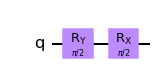
\includegraphics{Appendices/chapter_1/original_circuit_01.png}
            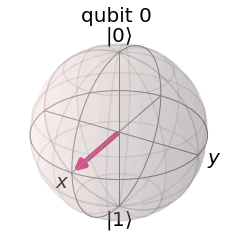
\includegraphics{Appendices/chapter_1/original_circuit_bloch_01.png}
            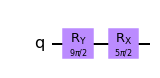
\includegraphics{Appendices/chapter_1/original_circuit_02.png}
            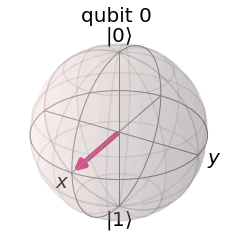
\includegraphics{Appendices/chapter_1/original_circuit_bloch_02.png}
        }
        \caption{Original unscaled data: Circuits and Bloch spheres of features which result in an identical state}
        \label{fig:unscaled_data_example}
    \end{subfigure}
    \\[4ex]
    \begin{subfigure}{1.0\textwidth}
        \scalebox{0.5}{
            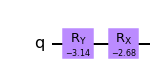
\includegraphics{Appendices/chapter_1/scaled_circuit_01.png}
            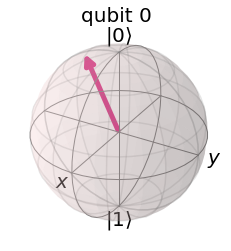
\includegraphics{Appendices/chapter_1/scaled_circuit_bloch_01.png}
            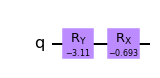
\includegraphics{Appendices/chapter_1/scaled_circuit_02.png}
            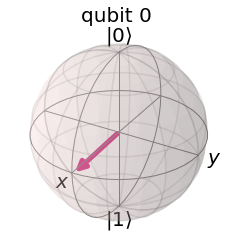
\includegraphics{Appendices/chapter_1/scaled_circuit_bloch_02.png}
        }
        \caption{Scaled data: Circuits and Bloch spheres of scaled features which result in a different state than the original data. In this example the same data - with additional data points that are not shown here - as in \ref{fig:unscaled_data_example} from above has been scaled using the \code{MinMaxScaler} with range $[-\pi,\pi]$.}
        \label{fig:scaled_data_example}
    \end{subfigure}
    \caption{Original versus scaled data example circuits and states}
    \label{fig:scaled_unscaled_data_example}
\end{figure}
